\documentclass[final, 10pt]{report}
\usepackage[utf8]{inputenc}
\usepackage[french]{babel}
\usepackage[top=2cm,bottom=2cm,left=2cm,right=2cm]{geometry}
\usepackage[style=numeric,backend=biber]{biblatex}
\usepackage{hyperref}
\usepackage{graphicx}
\usepackage[T1]{fontenc}
\usepackage{amssymb}
\usepackage{amsmath}
\usepackage{algpseudocode}
\usepackage{algorithm}
\usepackage{subcaption}

\setlength{\parskip}{5pt}

\addbibresource{Recherche_Documentaire_2022.bib}

\title{Recherche documentaire}
\author{CUENIN Tommy\and GROSDIDIER Alphée}
\date{January 2022}

\begin{document}

\maketitle

\tableofcontents

\chapter{Étude de différentes approches utilisées, sans rentrer dans des détails.}
\section{Introduction}
    %Ceci est un premier jet : il faut le retravailler
    Selon l'article de \emph{Wikipedia} \cite{noauthor_auto-completion_2019} \og\emph{L'auto-complétion ou autocomplétion ou complétion automatique, souvent simplement complétion, parfois complètement ou complètement automatique, est une fonctionnalité informatique permettant à l'utilisateur de limiter la quantité d'informations qu'il saisit avec son clavier, en se voyant proposer un complément qui pourrait convenir à la chaîne de caractères qu'il a commencé à taper.}\fg{}
    
    La complétion (semi-)automatique a pour but de nous simplifier la tâche d'écriture en corrigeant nos erreurs, en proposant différents mots suivant les premières lettres saisies ainsi qu'en nous proposant d'écrire des mots complets en 1 clic. 
    Elle permet une augmentation de la vitesse de saisie d'un texte et assure un respect des règles linguistiques de la langue choisie.
    
    Cette technologie est intégrée à toutes nos tâches d'écriture quotidiennes comme les rapports, mails, messages, ou encore l'écriture de code etc. Grâce à l'optimisation constante des programmes et à une meilleure compréhension du langage par les ordinateurs on est en mesure d'implémenter ces outils sur des appareils très peu puissants comme les téléphones portables tout en ayant une bonne efficacité.
    
    Présente sur la plupart des téléphones, elle augmente significativement la vitesse de saisie de texte en corrigeant les fautes de frappe et d'orthographe puis en recommandant des mots ce qui permet l'économie de la saisie de mots parfois longs. Cette vitesse est d'autant plus significative dans des langues où l'on peut écrire un mot composé en un seul bloc comme en allemand (par exemple :  die Messe + die Halle = die Messehalle  =  le hall d'exposition).


\section{Histoire}

    L’histoire des correcteurs automatiques a commencé chez \emph{Microsoft} au début des années 90, entre les mains d’un certain \emph{Dean Hachamovitch}.
    A cette époque le logiciel Word n'avais qu'un \og autoexpander\fg{}, des raccourcis clavier pour écrire un mot pré-enregistré.
    Alors \emph{Dean Hachamovitch} s'est inspiré de ce système pour créer premier mécanisme de correction connue.
    Ce logiciel remplaçais tous les \og teh\fg{} par \og the \fg{}.
    
    \emph{Hachamovitch} et son équipe ont vu que c'était une idée intéressante.
    Les années suivantes ils ont recensés les erreurs orthographiques et typographiques les plus courantes.
    Cependant le logiciel ne pouvais corriger que les fautes qui avais déjà été signalées et corrigées par l'équipe de \emph{Microsoft}.
    
    
    Le bouillonnement technologique de la fin des années 90 a vite apporté un début de solution au problème de Hachamovitch. Le fameux T9 ou « Texte sur neuf touches » de Cliff Kushler, le co-fondateur de l’entreprise Tegic Communications, mêlait le système de dictionnaire des logiciels de traitement de texte à des formules d’apprentissage des habitudes rédactionnelles des utilisateurs des premiers téléphones portables. La saisie intuitive était née. Taper des messages sur un clavier à neuf touches devenait soudain plus facile et rapide, juste à temps pour l’explosion de la popularité des SMS : en 1999, un Américain envoyait en moyenne 0,4 messages par mois… Et 35 cinq ans plus tard.
    \cite{wesolowski_les_2021}


\section{Par dictionnaire}

    La (semi-)complétion automatique par dictionnaire est la première approche a avoir été utilisé sur téléphone.
    A l'époque du \og T9\fg{} les applications pouvant tourner sur téléphones étaient très limitées en puissance de calcul et devait donc être peut gourmandes en ressources tout en restant rapide. 
    L'approche par dictionnaire est assez simple puisqu'il suffit d'un dictionnaire composés de tous les mots de la langue correctement orthographié et d'un bon algorithme de distance d'édition.
    
    
    Avec cette approche on vérifie si le mot est contenu dans le dictionnaire sinon on cherche le mot possible le plus proches avec le moins de caractères différents. 
    Dans l'exemple du T9 on met en priorité les changements avec les lettres qui sont sur les même touches. 
    Avec un clavier ce serais avec les touches qui se trouvent autour de la touche appuyé.
    
    
    On utilise aussi un dictionnaire utilisateur pour ajouter a la liste des mots correct les mots de l'utilisateur qui ne se trouvent pas dans le dictionnaire préfait.
    Cela permet d'être plus souple sur les corrections.
    
    Le problème lié a cette approche est que le dictionnaire de la langue doit être maintenu a jour très régulièrement. Ce qui rend difficile la maintenance du programme. De plus il est compliqué de répertorier tous les mots notamment le \og verlent \fg{} ou les mot raccourcis dans les \og textos \fg{}.
    
    Cette approche ne permet pas non plus de prendre en compte le contexte de la phrase ou du texte en générale ce qui rend cette approche limité. On peux l'utiliser pour corriger des mots mais une relecture humaine est obligatoire (bien que l'utilisation d'un correcteur orthographique doit souvent être suivie par une relecture).


\section{Par mot précédemment saisis}

    Ici on cherche a savoir quels mots on étés écrits et on suppose que l'utilisateur réécriras ces mots.
    En moyenne une personne française utilise 300 à 5000 mots\cite{admin6658_combien_2020} sur 32 000 mots couramment utilisées\cite{noauthor_combien_nodate} dans la langue française sur un total de 90 00 mots.
    On peux ainsi avoir de propositions de mots beaucoup plus rapide et juste en se basant simplement sur les 5000 mots que la personne utilisé.
    On peux lier une correction avec un dictionnaire des mots pour avoir une base des mots corrects écrits (puisqu'on veux corriger les textes) puis ensuite proposer les mots que l'utilisateur veux écrire avec son historique.
    
    Cependant cette approche pose le problème de savoir comment ses données vont êtres utilisée puisqu'elles sont enregistrées sur son téléphone mais pourrais très bien être récupérées par le créateur du logicielle.
    Ces données peuvent ensuite améliorer le logiciel ou être utilisée a des fin commerciales.
    

\section{Par les caractères de l'application}

    Certains mot ne sont utilisés que dans certains cas comme par exemple une adresse mail.
    Certains ne se trouve pas dans le dictionnaire et donc un logiciel de complétion (semi-)automatique auras des difficultés a les corriger.
    On a donc décider d'utiliser les informations des application pour compléter le dictionnaire de mot.
    Comme l'exemple cité précédemment l'application de mails va récupérer les mails enregistré pour corriger les adresses mails saisies.
    
    Sur les téléphones on utilise aussi cette approche pour les nom des contacts, en effet, les noms propres ne figurant pas dans le dictionnaire, ils seraient interprétés comme des erreurs et corrigés en vain. Cela permet à la fois d'éviter leur correction inutile ainsi que de corriger en cas d'erreur d'écriture du nom.
    %a développer

\section{Par sémantique}

    Avec l'amélioration de la puissance et de la mémoire du matérielle, une approche sur l'ensemble d'une phrase, voir d'un texte, a pus voir le jour.
    On décrira successivement les approches qui sont apparues pour pouvoir faire une prédiction de texte de plus en plus pertinente.
    
    \subsection{Algorithmes mathématiques}
    
        Dans les premier algorithmes, les chercheurs sont restée dans une approche plutôt mathématique.
        Ils ont eu une approche probabiliste en cherchant a savoir la fréquence a laquelle apparaissait une séquence qui en suivait une autre.
        % A continuer mais la j'ai plus le courrage
        
    
    \subsection{Intelligence artificielle}
    
        Une nouvelle approche qui a fais surface depuis quelques années est celle de l'intelligence artificielle.
        En théorie simple, elle reste une approche complique.
        Le principe est de travailler avec un réseau neuronal (On ne prendras pas le temps d'expliquer en détails leurs fonctionnement).
        On met en entrée les mots de la phrase et le réseau neuronal entraînée nous sort les meilleures mots pour compléter celle-ci.
        
        Mais on se retrouve face a plusieurs problèmes. 
        Dans un premier temps, si on prend en entrée les mots on a des dizaines de milliers d'entrées et de sorties ce qui est assez lourd pour le traitement.
        Puis pour les noms, qui sont spécifique a chaque utilisateur, n'ont pas forcément leur entrée ni leur sorties dans dans ce type d'intelligence artificielle.
        
        On serais donc tentées de prendre chaques lettre en entée et sortie mais le problème qui apparaît est que le risque d'avoir des mots qui n'existent pas dans la lanque.
        On a donc réfléchi a une autre approche en gardant l'intelligence artificielle qui promet de meilleure résultat que l'approche statique.
    
    \subsection{Algorithme GPT-3}


        L'algorithme GPT est développé par \textbf{OpenIA}, l’entreprise de recherche en IA co-fondée par Elon Musk\cite{noauthor_quest_2021}.
        Elle se base sur une réelle analyse sémantique cherchant a reconnaitre la valeur des mots.
        
        Par exemple dan la phrase: \og J'ai acheter du chocolat a Auchan pour le gâteau d'anniversaire de Jane \fg{}, l'algorithme reconnaîtras le mot \og Auchan \fg{} comme nom de marque et \og Jane \fg{} comme une personne.
        Cette analyse permet ensuite a un réseau neuronal de prédire la suite de la phrase de façon pertinente.
        Nous ne rentrons pas plus dans les détails mais il est important de noter que pour entraîner cet intelligence artificielle, cette organisation aurais dépensée près de 4,6 millions de dollars\cite{noauthor_quest_2021} et prendrais en compte 175 milliards de paramètres\cite{noauthor_quest_2021}.
        On est donc pas près de voir tourner cet algorithme sur nos téléphone portable autrement qu'a l'aide d'une connection avec une machine assez puissante.

\chapter{Étude des algorithmes de calcul de distance, par exemple de distance d’édition.}

\section{Algorithme de Levenshtein}

    L'algorithme de levensthein permet de calculer la distance entre deux chaînes.
    Elle quantifie la différence des deux chaînes de caractère. Et s'écrit sous forme mathématique $\text{lev}(C1,C2)$
    Pour ce faire elle dispose de trois opérations fondamentales qui sont~:
    \begin{itemize}
        \item l'ajout;
        \item la suppression;
        \item substitution de caractères.
    \end{itemize}
    
    \medskip
    Cet algorithme est considérée comme une généralisation de la distance de Hamming\cite{noauthor_distance_2021-1} qui était utilisée pour connaître le nombre de bits altérés lors de la transmission de messages dans les télécommunications.
    
    L'agorithme de Levensthein se définit par la formule suivante~:
    
    $$
    {\displaystyle \qquad \operatorname {lev} (a,b)={\begin{cases}\max(|a|,|b|)&{\text{ si }}\min(|a|,|b|)=0,\\\operatorname {lev} (a-1,b-1)&{\text{ si }}a[0]=b[0],\\1+\min {\begin{cases}\operatorname {lev} (a-1,b)\\\operatorname {lev} (a,b-1)\\\operatorname {lev} (a-1,b-1)\end{cases}}&{\text{ sinon.}}\end{cases}}}
     $$



Par exemple pour passer de "foyer" à "loyers", il faut effectuer deux opérations :
\begin{itemize}
    \item substitution du caractère 'f' par le caractère 'l'
    \item ajout du caractère 's'
\end{itemize}
La distance de Levenshtein dans ce cas est donc de 2.\\

À noter que chaque opération que l'on a cité a le même poids, qui est de 1 et que en toute logique dans le cas où les mots sont les mêmes la distance sera 0.\\

L'algorithme de Levenshtein est la formalisation en langage algorithmique du calcul de distance de Levenshtein,  à l'aide d'une matrice de taille $n$+$1\times m$+$1$ avec $n$ et $m$ la taille des deux mots dont l'on cherche la distance :\\

Voici ci-dessous un exemple d'utilisation de l'algorithme de Levenstein pour calculer la distance entre "foyer" et "loyers" :\\
\section{Algorithme de Damerau-Levensthein\cite{noauthor_distance_2020}}

    L'algorithme de Damereau-Levenstein utilise le même principe que l'algorithme de Levensthein.
    On garde les 3 opérations de base mais on ajoute une opération supplémentaire~: la transposition.
    La transposition est l'échange de position de deux lettre côte a côte qui a le même coût qu'une opération fondamentale.
    Ainsi le mot \fg chat \og{} et \fg hcat\fg{} ont un distance d'édition de 1 au lieu de 2 avec l'algorithme de Levensthein.
    
    Ces opérations forment environ 80\% des fautes d'orthographes humaines.
    On a donc un algorithme de correction orthographique qui est assez efficace mais on est encore loin d'avoir la perfection.
    \begin{figure}
        \centering
        \begin{subfigure}{0.4\textwidth}
            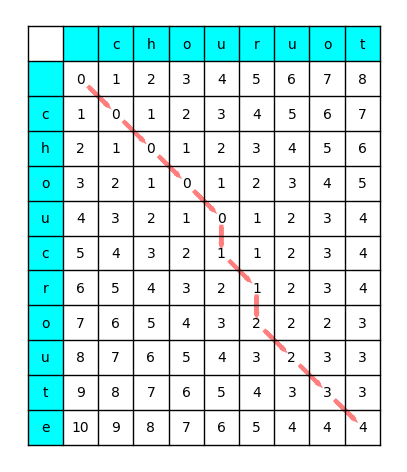
\includegraphics[height=0.4\textheight]{img/Tableau_de_Levenshtein.png}
            \caption{Tableau de Levensthein}
            \label{fig:tab_levensthein}
        \end{subfigure}
        \begin{subfigure}{0.4\textwidth}
            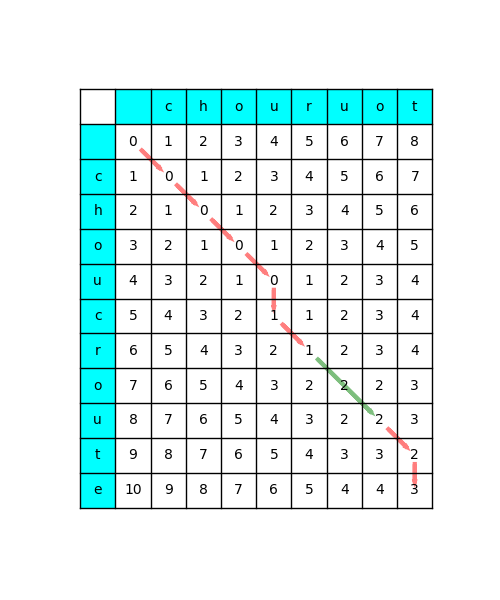
\includegraphics[height=0.4\textheight]{img/Tableau_de_Damerau-Levenshtein.png}
            \caption{Tableau de Damerau-Levensthein}
            \label{fig:tab_damerau}
        \end{subfigure}
        \caption{Algorithme type Levensthein}
        \label{fig:algo_levensthein}
    \end{figure}
    
\section{Algorithme de Jaro\cite{noauthor_distance_2021}}
    
    La distance de Jaro calcule le nombre de lettres qui sont présentes dans les deux mots et le nombre de lettres qui ne sont pas a la bonne place par rapport aux autres.
    
    %image
    
    On calcule la distance de Jaro a l'aide du calcul suivant~: 
    $$d_j = \frac{1}{3}\left(\frac{m}{\text{len}(c1)}+\frac{m}{\text{len}(c1)}+\frac{m-t}{m}\right)$$
    Où~:
    \begin{itemize}
        \item $\text{len}(ci)$ est la longeur de la chaine $i$;
        \item $m$ est le nombre de caractères correspondants;
        \item $t$ est le nombre de transpositions
    \end{itemize}

    \medskip
    On considère que deux caractères correspondent si le caractère est présent dans les deux chaîne et que la distance les séparant est inférieur ou égale a $$\lfloor\frac{\text{max}(\text{len}(c1), \text{len}(c2)}{2}\rfloor -1$$
    
\section{Algorithme de Jaro-Winker\cite{noauthor_distance_2021}}

    Une amélioration de l'algorithme de Jaro a été faite par William E. Winkler.
    Il a décidé de mettre plus d'importance sur la similitude des débuts de mot.
    
    On peux prendre l'exemple de \fg annuaire\og{} avec \fg annulaire\og{}. 
    La distance de jaro entre les deux mots est de $0.8630$.
    Maintenant si je compare  \fg annuaire\og{} avec \fg annnuaire\og{}.
    On a une distance de Jaro de $0.8630$.
    On a ajouter simplement une lettre dans les deux chaines.
    
    Les mots écrit humainement sont généralement bien écrit dans les premières lettre puis les fautes d'orthographes apparaissent.
    Donc pour être plus précis William E. Winkler a décidé d'avantager les mots qui ont le plus long préfixe commun.
    
    
    On a donc le calcul suivant~:
    $$ d_w = d_j +(l * p * (1-d_j) )$$
    Où~:
    \begin{itemize}
        \item $d_j$ est la valeur de l'algorithme de Jaro;
        \item $l$ est la longueur du préfixe commun (maximum 4 caractères);
        \item $p$ est un coefficient qui permet de favoriser les chaînes avec un préfixe commun.
        Winkler propose pour valeur $p=0.1$
    \end{itemize}
    
    Ainsi la distance Jaro-Winker entre \fg annuaire\og{} et \fg annulaire\og{} est de $0.9778$ alors que la distance entre \fg annuaire\og{} et \fg annnuaire\og{} est de $0.9741$
    
    Cet algorithme est plutôt utilisé dans la détection de doublons mais peut aussi être une approche dans la correction automatique
    
\chapter{Étude (simple) de chaînes de Markov pour l’historique.}

Une chaîne de Markov est un processus stochastique possédant la propriété de Markov, la propriété de Markov étant que, soit un système constitué de plusieurs états, fixé sur un état à la fois et pouvant transiter vers d'autre états, la prédiction de l'état futur du système à l'instant $n$ dépend uniquement de l'état du système à l'instant présent $n-1$ et donc est indépendante des états passés à l'instant $n-k$ avec $1<k\leq n$, donc le système n'a pas de mémoire.\\
Ainsi la probabilité de transition d'un état à l'autre dépend uniquement de l'état duquel on provient, on écrit donc la probabilité de transition $\mathbb{P}(X_{n+1}=a | X_{n}=b)$ avec $a$ et $b$ deux états pouvant être égaux.\\
\\
\begin{figure}[!h]
    \centering
    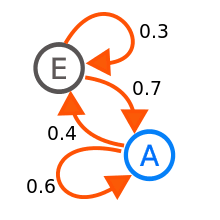
\includegraphics[scale=0.5]{img/markovChaine.png}
    \caption{Représentation d'une chaîne de Markov}
    \label{fig:chaine_markov}
\end{figure}
\\
Les chaînes de Markov sont modélisées en mathématiques par des matrices de transition qui sont des matrices carrées qui associe à chaque ligne un état initial et à chaque colonne la probabilité de transition vers un état, ainsi soit $(a,b)$ un couple d'entier et $M$ une matrice de transition, $M_{a,b}$ est la probabilité de transition de l'état numéro $a$ à l'état numéro $b$.\\
\\
La matrice de transition de la chaîne de Markov ci-dessus est la suivante (les lignes et les colonnes correspondent dans l'ordre aux états représentés sur le graphe E, A) : 
\\
$\begin{pmatrix}
0.3 & 0.7 \\
0.4 & 0.6
\end{pmatrix}$\\
\\
La somme des probabilités de chaque ligne doit être égale à 1 ce qui implique que tous les états doivent êtres connus ainsi que leur probabilité de transition.\\
\\
Les chaînes de Markov sont utilisées dans beaucoup de domaines, par exemple, les chaînes de Markov sont utilisées par Google pour déterminer l'indice de popularité d'une page web à partir d'un état quelconque de la chaîne de Markov représentant le Web.\\
\\
Dans le cas du sujet vu qu'un texte est une suite de mots, on pourrait partir du principe qu'un mot est un état.
Si on se sert de chaque saisie d'utilisateur pour compléter des chaînes de Markov associées on pourrait déterminer quels sont les mots les plus fréquemment utilisés à la suite d'un autre et ainsi faire des propositions intéressantes car se basant sur la fréquence.\\
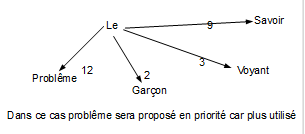
\includegraphics[scale=1]{img/Mark.png}\\
Cependant cette approche a des limites comme l'absence de mémoire qui empêche d'affiner la recommandation de mots car cette dernière se base sur uniquement un seul mot et non l'ensemble de la phrase qui précède.
\chapter{Programmer un petit outil de ce type en s’appuyant sur différentes techniques.}
%Parler de pourquoi on a choisis de faire comme on a fait

\printbibliography

\end{document}

